\section{CFG Basics}

\begin{itemize}
 
\item The maximal basic blocks are outlined below. 


\begin{table}[!ht]
\centering
\begin{tabular}{l l l }
  \toprule
  \toprule
Basic Block Label & & Code \\
\midrule
B1 & & \shortstack[l]{x = 50 \\ y = 8 \\ if (x $>$ y) goto L2} \\
\midrule
B2 & & \shortstack[l]{x = 50 \\ goto L3} \\
\midrule
B3 & L1: & \shortstack[l]{x = 27 \\ return x}\\
\midrule
B4 & L2: & \shortstack[l]{y = x + 1 \\ if (y $<$ x) goto L2}\\
\midrule
B5 &  & x = 24\\
\midrule
B6 & L3: & \shortstack[l]{z = x + y \\ switch (z) \{ 26 $=>$ L1 $\|$ 32 $=>$ L4 $\|$ default $=>$ L5 \} } \\
\midrule
B7 & L4: & print(``success'') \\
\midrule
B8 & L5: & \shortstack[l]{x = 50\\return x}\\
\bottomrule
\end{tabular}
\end{table}

\item The CFG is given in Figure~\ref{fig:cfg}.
  
\begin{figure}
\centering
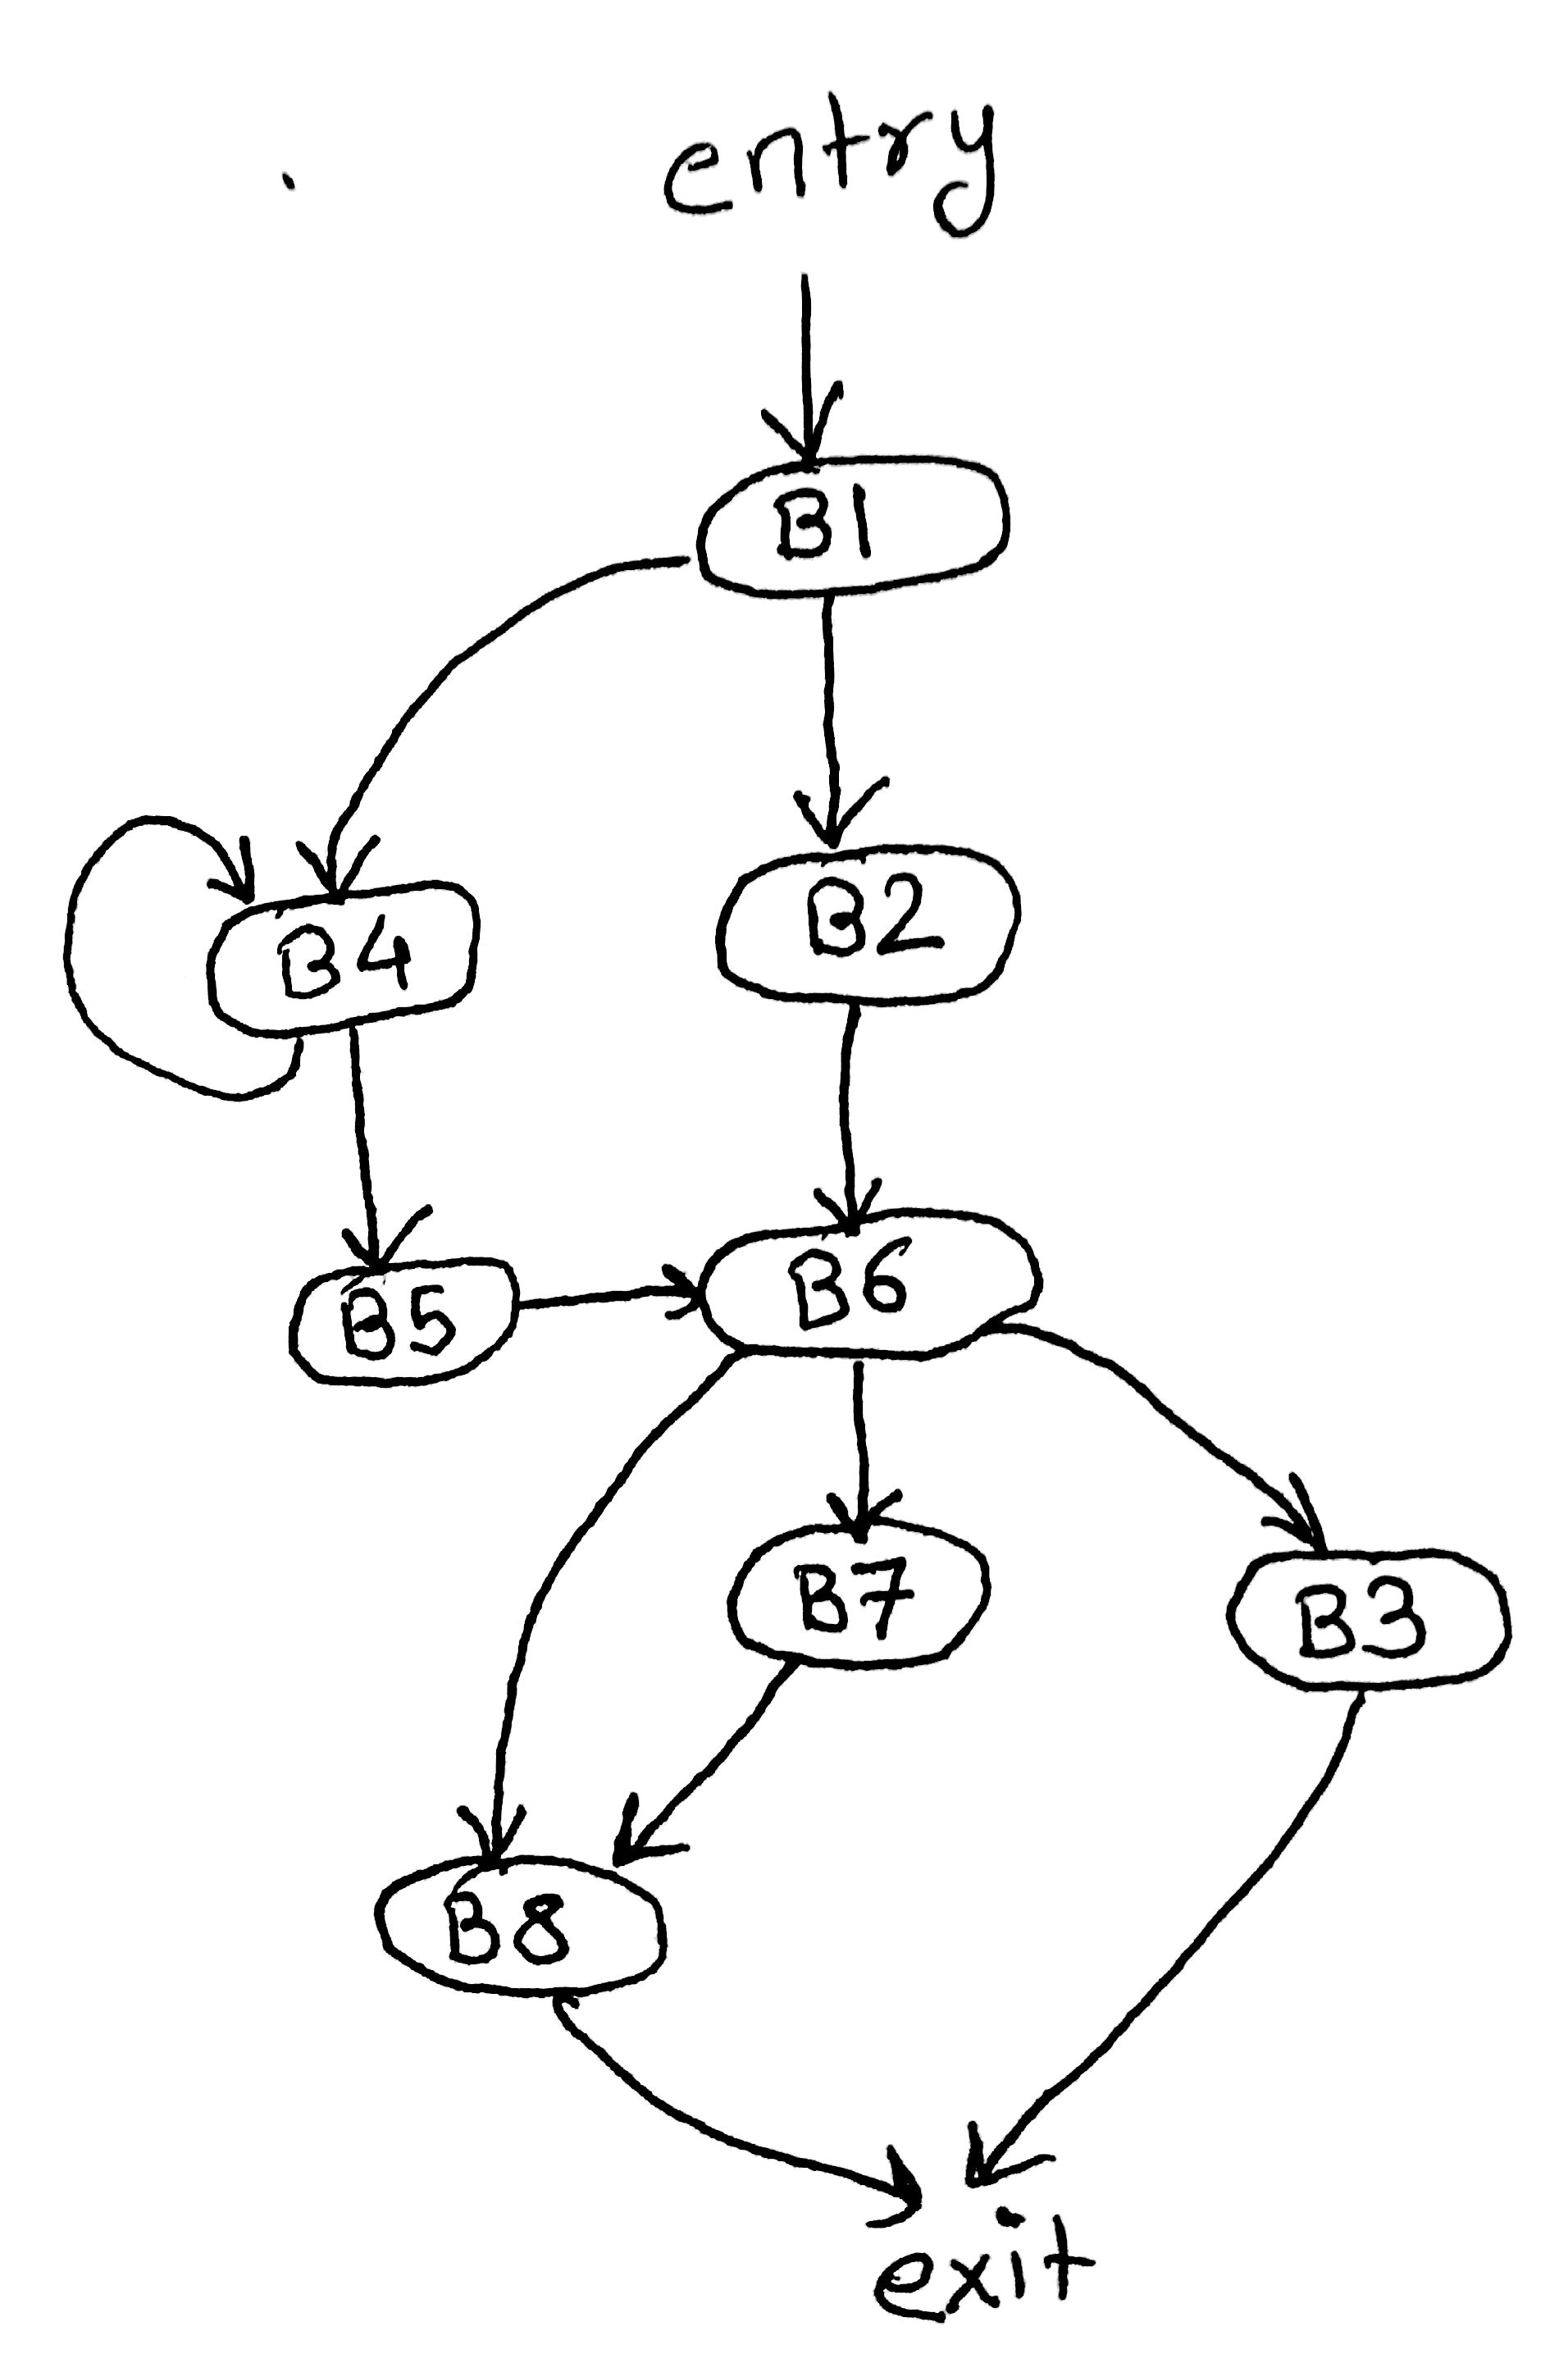
\includegraphics[width=0.7\textwidth]{images/CFG.jpg}
\caption{CFG}
\label{fig:cfg}
\end{figure}

\end{itemize}
